\chapter{Variétés}
   Dans toute la suite, on considère un espace topologique compact et séparé \( M \).
   \section{Cartes locales}
      On apelle \textbf{carte locale} de \( M \) un couple \( (U, \phi) \) tel que:
      \begin{itemize}
         \item \( U \) soit un \textbf{ouvert} de \( M \).
         \item \( \phi \) soit un \textbf{homéomorphisme} de \( U \longrightarrow \phi(U) \subseteq \R^n \) pour un \( n \) convenable.
      \end{itemize}
      On dira alors que l'application \( \phi^{-1} \) paramétrise \( U \), et que les \textbf{coordonées locales} des points de \( U \) sont leurs images par \( \phi \).\<

      On apelle alors \textbf{atlas} de \( M \) une famille \(\mathcal{A} = (U_i, \phi_i)_{i \in I}\) de cartes locales qui recouvrent \( M \). Alors si un tel atlas existe on dira que l'espace \( M \) est une \textbf{variété topologique}.
   \section{Structure différentielle}
   On souhaite alors enrichir la structure de variété, et à terme munir \( M \) d'une structure permettant de différentier des fonctions sur celle-ci. On définit pour deux cartes \( (U_i, \phi_i), (U_j, \phi_j) \) qui s'intersectent la notion de cartes \( \mathcal{C}^k \)-\textbf{compatibles} si et seulement si l'application suivante est de classe \( \mathcal{C}^k \):
   \[ 
      \phi_{ij} = \phi_j \circ \phi_i^{-1} : \phi_i(U_i \cap U_j) \longrightarrow \phi_j(U_i \cap U_j)
   \]
   L'application \( \phi_{ij} \) est apellée \textbf{application de changement de cartes}, on peut la représenter comme ci-dessous:

   \begin{figure}[H]
      \centering
         \begin{tikzpicture}[scale=0.95,]
            \path[->] (0.8, 0) edge [bend right] node[left, xshift=-2mm] {$\phi_i$} (-1, -2.9);
            \draw[white,fill=white] (0.06,-0.57) circle (.15cm);

            \path[->] (4.2, 0) edge [bend left] node[right, xshift=2mm] {$\phi_j$} (6.2, -2.8);
            \draw[white, fill=white] (4.54,-0.12) circle (.15cm);
        
            % Manifold
            \draw[smooth cycle, tension=0.4, fill=white, pattern color=white, pattern=north west lines, opacity=0.7] plot coordinates{(2,2) (-0.5,0) (3,-2) (5,1)} node at (3,2.3) {$M$};
        
            % Help lines
            %\draw[help lines] (-3,-6) grid (8,6);
        
            % Subsets
            \draw[smooth cycle, pattern color=BrightRed1, pattern=north east lines] 
                plot coordinates {(1,0) (1.5, 1.2) (2.5,1.3) (2.6, 0.4)} 
                node [label={[label distance=-0.3cm, xshift=-2cm, fill=white]:$U_i$}] {};
            \draw[smooth cycle, pattern color=BrightBlue1, pattern=north west lines] 
                plot coordinates {(4, 0) (3.7, 0.8) (3.0, 1.2) (2.5, 1.2) (2.2, 0.8) (2.3, 0.5) (2.6, 0.3) (3.5, 0.0)} 
                node [label={[label distance=-0.8cm, xshift=.75cm, yshift=1cm, fill=white]:$U_j$}] {};
        
            % First Axis
            \draw[thick, ->, >=stealth] (-2.5,-5) -- (-0.25, -5);
            \draw[thick, ->, >=stealth] (-2.5,-5) -- (-2.5, -2.5);
        
            % Arrow from i to j
            \draw[->] (0, -3.85) -- node[midway, above]{$\phi_j \circ \phi_i^{-1}$} (4.5, -3.85);
        
            % Second Axis
            \draw[thick, ->, >=stealth] (5.25, -5) -- (7.5, -5);
            \draw[thick, ->, >=stealth] (5.25, -5) -- (5.25, -2.5);
        
            % Sets in R^m
            \draw[white, pattern color=BrightRed1, pattern=north east lines] (-0.67, -3.06) -- +(180:0.8) arc (180:270:0.8);
            \fill[even odd rule, white] [smooth cycle] plot coordinates{(-2, -4.5) (-2, -3.2) (-0.8, -3.2) (-0.8, -4.5)} (-0.67, -3.06) -- +(180:0.8) arc (180:270:0.8);
            \draw[smooth cycle] plot coordinates{(-2, -4.5) (-2, -3.2) (-0.8, -3.2) (-0.8, -4.5)};
            \draw (-1.45, -3.06) arc (180:270:0.8);
        
            \draw[white, pattern color=BrightBlue1, pattern=north west lines] (5.7, -3.06) -- +(-90:0.8) arc (-90:0:0.8);
            \fill[even odd rule, white] [smooth cycle] plot coordinates{(7, -4.5) (7, -3.2) (5.8, -3.2) (5.8, -4.5)} (5.7, -3.06) -- +(-90:0.8) arc (-90:0:0.8);
            \draw[smooth cycle] plot coordinates{(7, -4.5) (7, -3.2) (5.8, -3.2) (5.8, -4.5)};
            \draw (5.69, -3.85) arc (-90:0:0.8);    
         \end{tikzpicture}
         \hfill
         \caption{Exemple de deux cartes}
   \end{figure} 
   En outre si \( M \) est muni d'un atlas tel que deux cartes sont systématiquement \( \mathcal{C}^k \)-compatibles, on dira que \( M \) est une \textbf{variété différentielle} (ou encore d'une structure différentielle) de classe \( \mathcal{C}^k \).
   \section{Notion de différentiabilité}
   Etant donné une application \( f : M \longmapsto \R \), la structure différentielle nous permet alors de généraliser la définition de différentiabilité dans \( \R^n \) à une notion de différentiabilité dans \( M \) en un point \( x \), en effet pour \( (U, \phi) \) une carte qui contient \( x \), on donne la définition suivante:
   \begin{center}
      \( f \) est \textbf{différentiable} en \( x \) si et seulement si \( f \circ \phi^{-1} \) est \textbf{différentiable} en \( \phi(x) \)
   \end{center}
   De manière plus générale on dira pour une application \( f : M \longmapsto N \), une carte \( (U, \phi) \) qui contient \( x \) et une carte \( (V, \psi) \) qui contient \( f(x) \) alors on définit:
   \begin{center}
      \( f \) est \textbf{différentiable} en \( x \) si et seulement si \( \psi \circ f \circ \phi^{-1}\) est \textbf{différentiable} en \( \phi(x) \)
   \end{center}
   Ces deux définitions nécessitent alors de vérifier que ceci ne dépends pas des cartes choisies, et donc (dans le premier cas) que \( f \circ \phi^{-1} \) est différentiable si et seulement si \( f \circ \psi^{-1} \) est différentiable. Ceci est vrai \textbf{exactement} gràce à la contrainte de régularité des application de changement de carte.
   \section{Partition de l'unité subordonnée à l'atlas}
      Alors un des résultats fondamentaux pour construire la théorie de l'intégration sur une variété est le suivant:
      \begin{center}
         \textbf{Il existe une partition de l'unité lisse subordonnée à l'atlas.}
      \end{center}
      L'existence de telles partitions repose sur l'existence de \textbf{fonctions bosse lisses}, ie de fonctions à support compact et identiquement égales à 1 sur un ouvert inclu dans leur support.

\chapter{Variétés à bord}
   On veut alors pouvoir relaxer cette définition pour prendre en compte une catégorie plus large d'espaces topologiques, en particulier si on considère le disque ouvert \( D^1 \), c'est trivialement\footnote[1]{Comme graphe d'une fonction constante définie sur un ouvert.} une variété, mais le disque fermé \( \text{adh}(D^1) \) ne l'est pas. La différence fondamentale étant qu'un ouvert qui contient un point du bord du disque fermé n'est pas homéomorphe à un ouvert de \( \R^2 \) Mais à un ouvert du demi-plan \( \R \times \R_+ \).

   \section{Bord du demi-espace \( \R^n_+ \)}
   On note \( \R^n_+ := \left\{ x \in \R^n  \; ; \; x_n \geq 0\right\} \). Cet espace sera notre prototype de partie avec un bord, en effet si on considère cet espace en tant que partie de \( \R^n \), son bord est bien défini:
   \[ 
      \partial \R^n_+ := \R^n_+ \backslash \text{int}(\R^n_+) = \left\{ x \in \R^n \; ; \; x_n = 0\right\}  
   \]
   Par exemple dans le cas de \( \R^2_+ \), on a:
      \begin{figure}[ht!]
         \centering
         \begin{tikzpicture}
            % Hachures pour x < 0
            \fill[pattern=north east lines, pattern color=black!50] (-2,-2) rectangle (0,2);
            
            \draw[line width = 0.8] (-2,0) -- (2,0);
            \draw[color=BrightRed1, line width = 1.5] (0,-2) -- (0,2) node[below right] {$\partial \mathbb{R}^2_+$};
            \draw[color=BrightRed1, line width = 1.5] (0,-2) -- (0,2);
        \end{tikzpicture}
        \caption{Le demi plan \( \R^2_+ \) et son bord}
      \end{figure}
   \vspace{-15pt}
   \section{Variété à bord}
   On donne élargit alors notre définition d'une variété, qui sera notre définition générale pour la suite. On se donne une variété \( M \) muni de son atlas \( (U_i, \phi_i)_{i \in I} \) et on rajoute la contrainte suivante sur les cartes:
   \[ 
      \forall i \in I \; ; \; \phi_i : U_i \longmapsto V_i \text{ avec } V_i \text{ un ouvert de } \R^n_+
   \]
   Ceci nous permet de définir le bord d'une variété par:
   \[ 
      \partial M := \left\{ x \in M  \; ; \; \exists (U, \phi) \in \mathcal{A} \; ; \; x \in U \text{ et } \phi(x) \in \partial\R^n_+\right\}  
   \]
   Alors on peut montrer que c'est bien une généralisation du concept de variété, en effet si une variété définie de la sorte n'a pas de bords, ie si \( \partial M = \emptyset\), alors on peut construire un atlas au sens du chapitre 2.\<

   En particulier, on peut remarquer que \( \R^n_+ \) lui-même est bien une variété à bord ce qui est bien cohérent ...
\chapter{Exemples de variétés}
   Dans ce chapitre, on présente quelques exemples simples de variétés différentielles, leurs atlas et quelques unes de leurs propriétés.
   \section{Variété triviale}
   On considère l'espace topologique \( \widetilde{\R^2} = \R^2 \backslash D\) où \(D = \left\{ (x, y) \in \R^2 \; ; \; x < 0 \right\}\), alors il est muni de la carte triviale cartésienne de \( \R^2 \) par définition. On peut aussi considérer la carte (globale) polaire, on a donc deux cartes:
   \[ 
      \begin{aligned}
         \phi : \widetilde{\R^2} &\longrightarrow \widetilde{\R^2} \\
         (x, y) &\longmapsto (x, y)
      \end{aligned} \quad\quad
      \begin{aligned}
         \psi^{-1} : \ioo{0}{+\infty} \times \ioo{-\pi}{\pi} &\longrightarrow \widetilde{\R^2} \\
         (r, \theta) &\longmapsto (r \cos( \theta), r \sin( \theta))
      \end{aligned}
   \]
   Alors l'application de changement de carte est facilement donnée par \( \psi^{-1} \) qui est bien un difféomorphisme. Ceci démontre alors que \( \widetilde{\R^2} \) muni de la carte cartésienne et polaire est muni d'une structure de variété différentielle. 
   \section{Variétés simples}
   On peut montrer facilement que tout les objets suivants sont des variétés différentielles:
   \begin{itemize}
      \item Les \textbf{graphes de fonctions lisses}.
      \item Les \textbf{courbes paramétrées} par une application lisses et sans points critiques.
   \end{itemize}
   \section{Le cercle \( \mathbb{S}^1 \)}
   On considère le cercle unité \( \mathbb{S}^1 \), alors il existe de multiples manière de munir cet espace topologique d'une structure différentielle. La plus élégante consiste à fixer \( N, S \) le pôles nord et sud du cercle et à considèrer les deux cartes correspondant à la \textbf{projection stéréographique} passant par ces points.
   \begin{figure*}[h]
      \centering
      \begin{tikzpicture}  
         % Définitions des variables
         \def\R{2} % Rayon du cercle
         \def\xp{1.2} % Coordonnée x du point P sur le cercle
         \def\yp{sqrt(\R*\R - \xp*\xp)} % Calcul de y pour rester sur le cercle
         \def\xpp{\xp / (1 - \yp/\R)} % Coordonnée x de P' par projection
         \def\ypp{0} % P' est sur l'axe x

         % Dessin du cercle
         \draw[thick] (0,0) circle (\R);
         
         % Axe horizontal (plan de projection)
         \draw[thick, dashed] (-7,0) -- (7,0);
         \draw[thick, dashed] (0,-2) -- (0,2);

         % Pôle nord
         \fill[black] (0,\R) circle (2pt) node[above] {$N$};

         % Point P sur le cercle
         \fill[] ({\xp},{\yp}) circle (2pt) node[above right] {$(x,y)$};
         % Projection P' sur l'axe x
         \fill[] ({\xpp},{\ypp}) circle (2pt) node[below] {$p_N(x,y)$};
         % Projection (lignes)
         \draw[dashed, thick] ({\xp},{\yp}) -- (0,\R); % Ligne vers le pôle nord
         \draw[thick] ({\xp},{\yp}) -- ({\xpp},{\ypp}); % Projection
      \end{tikzpicture}
      \caption{Projection stéréographique via le pôle Nord}
   \end{figure*}

   Alors, des faits géométriques élémentaires permettent de trouver l'expression analytique de ces deux projections:
   \[ 
      \begin{aligned}
         p_N : \mathbb{S}^1 &\longrightarrow \R \\
         (x, y) &\longmapsto \frac{x}{1-y}
      \end{aligned} \quad\quad
      \begin{aligned}
         p_S : \mathbb{S}^1 &\longrightarrow \R \\
         (x, y) &\longmapsto \frac{x}{1+y}
      \end{aligned}
   \]
   Alors on vérifie que ces deux applications sont des homéomorphismes sur leur image, d'inverses:
   \[ 
      \begin{aligned}
         p_N^{-1} : \R &\longrightarrow \mathbb{S}^1 \\
         x &\longmapsto \left(\frac{2x}{x^2+1}, \frac{1-x^2}{x^2+1}\right)
      \end{aligned} \quad\quad
      \begin{aligned}
         p_S^{-1} : \R &\longrightarrow \mathbb{S}^1 \\
         x &\longmapsto \left(\frac{2x}{x^2+1}, \frac{x^2-1}{x^2+1}\right)
      \end{aligned}
   \]
   Ceci munit le cercle d'une structure de variété topologique, en outre on peut montrer que les applications de changement de cartes sont différentiables. Et donc le cercle est bien muni d'une structure différentielle.
   \section{La sphere \( \mathbb{S}^2 \)}
   On considère la sphère unité \( \mathbb{S}^2 \), alors il existe de multiples manière de munir cet espace topologique d'une structure différentielle. La plus élégante consiste à nouveau à fixer \( N, S \) le pôles nord et sud de la sphère et à considèrer les deux cartes correspondant à la \textbf{projection stéréographique} passant par ces points.
   \begin{figure*}[h]
      \centering
         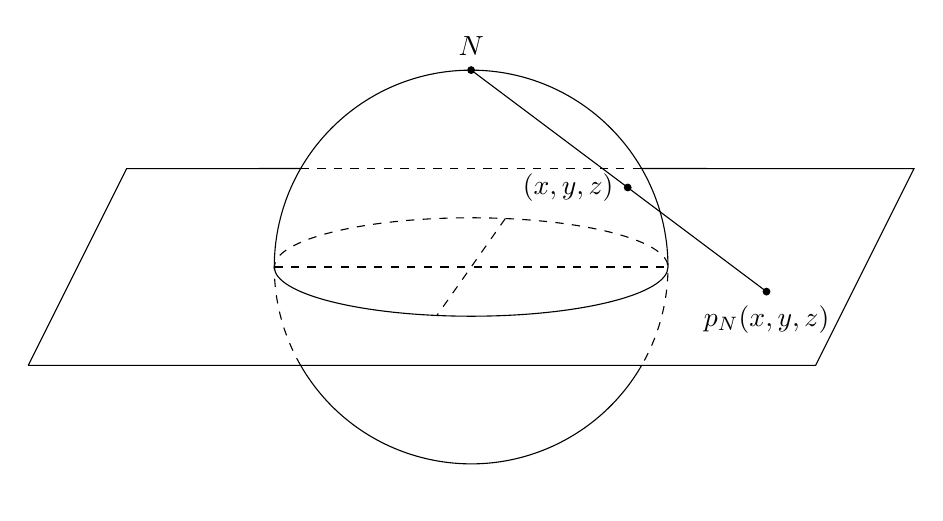
\begin{tikzpicture}[scale=1.25]
            \coordinate (A) at (3,-0.25);
            \coordinate (P) at (0,2);
      
            \draw (0:2cm)   arc[radius=2cm,start angle=0,end angle=180]
                  (210:2cm) arc[radius=2cm,start angle=210,end angle=330];
            \draw (180:2cm) arc[x radius=2cm, y radius=0.5cm, start angle=180,end angle=360];
      
            \draw [dashed] (210:2cm) 
                  arc[start angle=210,delta angle=-30,radius=2cm]
                  arc[start angle=180,delta angle=-180,x radius=2cm,y radius=0.5cm]
                  arc[start angle=0,delta angle=-30,radius=2cm];
      
            \draw [dashed] (80:2cm and 0.5cm) -- (260:2cm and 0.5cm);
            \draw [dashed] (150:2cm) coordinate(ul) -- (30:2cm) coordinate(ur);
      
            \draw (-4.5,-1) -- (3.5,-1) -- (4.5,1) -- (ur) (ul) -- (-3.5,1) -- (-4.5,-1);
      
            \draw (A) -- (P) coordinate[pos=0.47](B);
            \path (A) node[circle, fill, inner sep=1pt, label=below:{$ p_N(x,y,z) $}]{};
            \path (B) node[circle, fill, inner sep=1pt, label=left:{$ (x, y, z) $}]{};
            \path (P) node[circle, fill, inner sep=1pt, label=above:{$N$}]{};
            \draw [dashed] (-2,0) -- (2,0);
         \end{tikzpicture}
      \caption{Projection stéréographique de la sphère par rapport au pôle Nord}
   \end{figure*}
   On peut alors de manière analogue au cercle, trouver l'expression analytique des deux projections et montrer qu'elles munissent \( \mathbb{S}^2 \) d'une structure de variété différentielle.
\chapter{Espaces tangents dans \( \R^n \)}
   On aimerait alors pouvoir généraliser la notion \textbf{d'espace tangent} à une courbe, surface ... lisse de \( \R^n \) à des variétés abstraites comme définies dans les deux premiers chapitres. Pour ce faire, il est fondamental de comprendre que les variétés ainsi définies ne sont \textbf{pas} des objets de \( \R^k \), donc la notion de vecteur tangent géométrique perd son sens.\<

   L'approche fructueuse consiste alors à identifier \textbf{vecteurs} de \( \R^n \) et \textbf{dérivations} via la notion de dérivée directionnelle. On considère tout d'abord le cas de \( \R^n \), puis on généralise dans une variété quelconque.
   \section{Notion de dérivation:}
      Soit \(p \in \R^n\), on dira qu'un opérateur linéaire \( D: \mathcal{C}^\infty(\R^n) \longrightarrow \R \) est une \textbf{dérivation} en \( p \) si et seulement si elle vérifie la \textbf{règle de Leibniz} donnée par:
      \[ 
         D(fg) = D(f)g(p) + f(p)D(g) 
      \]
      En particulier, les opérateurs de dérivées partielles d'une fonction lisse sont des dérivations. On peut aussi facilement montrer que si \( f \) est constante \( Df = 0 \) pour toute dérivation \( D \).
   \section{Espace tangent \( T\R^n_p \):}
      On appelle alors \textbf{espace tangent} à \( \R^n \) en \( p \) l'ensemble \( T\R^n_p \) de toutes les dérivations en \( p \) de fonctions lisses. On pose alors l'application suivante:
      \[ 
         \begin{aligned}
            \Phi : \R^n &\longrightarrow T\R^n_p \\
            v &\longmapsto \sum_{i \leq n} v_i \partialD{}{x_i}\biggr|_p
         \end{aligned} 
      \]
      Où les \( v_i \) sont les coordonées de \( v \) dans la base canonique. Alors on montre la propriété fondamentale qui est que \( \Phi \) est un \textbf{isomorphisme}. Ceci nous permet alors d'identifier vecteurs et dérivations, en outre, on en déduit une base de \( T\R^n_p \) qui est alors donnée par:
      \[ 
         \Phi(e_i) = \partialD{}{x_i}\biggr|_p
      \] 
      Les "vecteurs" ainsi définis agissent sur les fonctions lisses par dérivation directionelle, en effet si on considère par exemple \( v = \partialD{}{x}\big|_{(x, y)} + 2\partialD{}{y}\big|_{(x, y)}\) et \( f(x, y) = xy \), alors on peut définir:
      \[ 
         vf = \partialD{f}{x}(x, y) + 2\partialD{f}{y}(x, y) = y + 2x
      \]
\chapter{Espaces tangents sur une variété}
   On généralise l'approche du chapitre précédent au cas des variétés, et on en déduit une définition de l'espace tangent en un point, intrinsèque et qui ne dépends pas des cartes. Dans toute la suite, on considèrera une fonction \( f : M \longrightarrow N \) point \( p \in M \), une carte \( \phi = (x_1, \ldots, x_n) \) et \( \psi = (y_1, \ldots, y_n) \) qui contiennent respectivement \( p \) et \( f(p) \)
   \section{Espace tangent en un point:}
      On définit une \textbf{dérivation} sur \( M \) en un point \( p \) comme un opérateur linéaire sur \( \mathcal{C}^\infty(M) \) qui vérifie la règle de Leibniz. On définit alors de manière analogue au cas euclidien \( TM_p \) comme l'ensemble des telles dérivations. C'est alors un espace vectoriel pour les lois usuelles.
   \section{Différentielle}
      On considère alors une application lisse \( f : M \longmapsto N \) et \( p \in M \). On définit alors la \textbf{différentielle} de l'application \( f \) en \( p \) par l'application suivante:
      \[ 
         \begin{aligned}
            df_p : TM_p &\longrightarrow TN_{f(p)} \\
            D &\longmapsto \left( g \longmapsto D(g \circ f) \right)
         \end{aligned} 
      \]
      C'est moralement une application qui transporte les dérivations. On peut alors vérifier que cette application est bien définie et qu'elle vérifie les propriétés suivantes:
      \begin{itemize}
         \item Elle est \textbf{linéaire}.
         \item Elle vérifie la \textbf{règle de la chaîne:} \( d(f \circ g)_p = df_{g(p)} \circ dg_p \)
         \item Si \( f \) est un \textbf{difféomorphisme}, alors \( \forall p \in M \; ; \; df_p \) est un \textbf{isomorphisme}.
      \end{itemize}
      On peut alors montrer que pour ces définitions, si on considère une carte \( (U, \phi) \) qui contient \( p \), alors c'est un \textbf{difféomorphisme} et donc on a l'isomorphisme suivant:
      \[ 
         \begin{aligned}
            d\phi_p : TM_p &\longrightarrow T\R_{\phi(p)}^n
         \end{aligned} 
      \]
      On en déduis donc que \( TM_p \) est un espace vectoriel de dimension \( n \) et qu'une base  est donnée par:
      \[ 
         \partialD{}{x_i}\biggr|_p := d\phi^{-1}\left( \partialD{}{x_i}\biggr|_{\phi(p)}\right) 
      \]
      Ce sont des dérivations dont l'action sur une fonction lisse\footnote[1]{Si \( f : M \longrightarrow N \) alors on peut aussi définir une action de ces dérivées partielles en composantes en notant \( f_j(p) = (\psi \circ f)_j(p) \) la \( j \)-ième composante de \( f \), et alors \( \partialD{}{x_i}\bigr|_p(f) := \left(\partialD{}{x_i}\bigr|_p(f_1), \ldots,  \partialD{}{x_i}\bigr|_p(f_n)\right) \)} \( f \) est définie par la dérivation partielle dans les coordonées locales:
      \[ 
         \partialD{}{x_i}\biggr|_pf = \partialD{f \circ \phi^{-1}}{x_i}(\phi(p))
      \]
      \pagebreak
   \section{Changement de représentation des vecteurs tangents}
      Dans la section précédente on a défini une représentation en coordonées locales d'un vecteur de l'espace tangent \( TM_p \), une question naturelle est alors:
      \begin{center}
         \textit{Quel est le lien entre deux telles représentations dans deux cartes différentes ?}
      \end{center}
      On peut alors montrer la propriété suivante si \( (U, \phi), (V, \psi) \) sont deux cartes qui contiennent un point \( p \), alors si on note \( x_i, y_i \) les coordonées respectives dans la première et la deuxième carte et \( c = \psi \circ \phi^{-1} \) l'application de changement de carte alors:
      \begin{align*}
         \partialD{}{x_i}\biggr|_p &= \sum_{j \leq n} \partialD{c_j}{x_i}(\phi(p)) \partialD{}{y_j}\biggr|_p
      \end{align*}
   \section{Fibré tangent}
   On cherche alors a globaliser la notion d'espace tangent ponctuel et considérer \textbf{l'ensemble de tout les espaces tangents}. Ce point de vue est fructueux car il permettra de définir de manière simple la notion de champs de vecteurs sur une variété. On appelle cet ensemble le \textbf{fibré tangent} de \( M \) et il est défini par:
   \[ 
      TM = \bigsqcup_{p \in M} TM_p = \bigcup_{p \in M} \{p\} \times TM_p
   \]
   \begin{figure}[h]
      \centering
      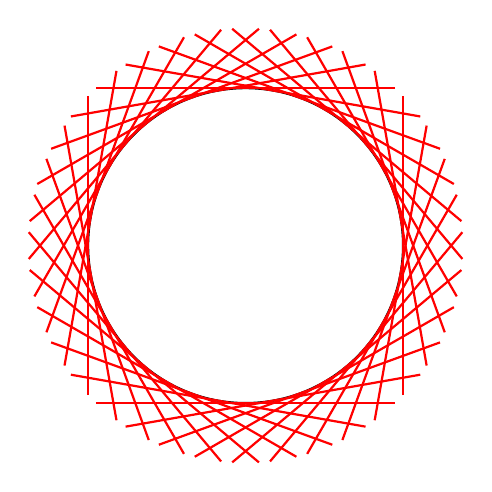
\begin{tikzpicture}
         % Dessiner le cercle
         \draw[thick] (0,0) circle (2);
         
         % Définir des points sur le cercle et leurs tangentes
         \foreach \angle in {10, 20, 30, 40, 50, 60, 70, 80, 90, 100, 110, 120, 130, 140, 150, 160, 170, 180, 190, 200, 210, 220, 230, 240, 250, 260, 270, 280, 290, 300, 310, 320, 330, 340, 350, 360} {
            % Calcul des coordonnées du point sur le cercle
            \pgfmathsetmacro\x{2*cos(\angle)}
            \pgfmathsetmacro\y{2*sin(\angle)}
            
            % Calcul du vecteur tangent (perpendiculaire au rayon)
            \pgfmathsetmacro\tx{-sin(\angle)}
            \pgfmathsetmacro\ty{cos(\angle)}
            
            % Tracer une droite tangentielle passant par le point
            \draw[red, thick] 
               ({\x - 1.9*\tx}, {\y - 1.9*\ty}) -- 
               ({\x + 1.9*\tx}, {\y + 1.9*\ty});
         }
      \end{tikzpicture}
      \caption{Fibré tangent du cercle \( \mathbb{S}^1 \)}
   \end{figure}

   Le fibré tangent hérite alors de plusieurs propriétés:
   \begin{itemize}
      \item Une projection \( \pi : (p, v) \in TM \mapsto p\) qui projete chaque vecteur sur son point base.
      \item Une topologie définie par la préimage de celle ci.
   \end{itemize}
   De ces propriétés, on peut alors montrer que \( TM \) peut être muni d'une structure de \textbf{variété différentielle} de dimension \( 2n \). En effet on considère une carte \( (U, \phi) \) de \( M \), alors on pose:
   \[ 
      \left(\pi^{-1}(U), (p, v) \mapsto (\phi(p), d\phi_p(v)) \right)
   \]
   Alors en identifiant \( T\R^n_p \cong \R^n \), ceci définit une carte locale sur l'ouvert \(\pi^{-1}(U)\) et on peut alors montrer que l'ensemble des cartes ainsi construites forme bien un atlas sur \( TM \).\<

   Un des intérêts de cette notion est qu'on peut alors identifier la différentielle comme une application globale sur les fibrés donnée par:
   \[ 
      \begin{aligned}
         df : TM &\longrightarrow TN \\
         (p, v) &\longmapsto (f(p), df_p(v))
      \end{aligned} 
   \]
   En fait, les cartes de \( TM \) sont exactement les différentielles globales de celles ci ?
   \section{Champs de vecteurs}
   On peut alors définir la notion de \textbf{champs de vecteurs} sur une variété \( M \) par la donnée d'une application lisse de la forme:
   \[ 
      \begin{aligned}
         V : M &\longrightarrow TM \\
         p &\longmapsto (p, v)
      \end{aligned} 
   \]
   Où on identifiera \( V(p) \triangleq v \). Alors plus précisément, si on fixe \( p \in M \), alors en coordonées locales on a:
   \[ 
      V(p) = \sum_{i = 1}^n V_i(p) \partialD{}{x_i}\biggr|_p
   \]
   Un tel champs de vecteurs est dit lisse au sens d'une application lisse entre les variétés \( M \) et \( TM \), on note alors $\mathfrak{X}(M) $ l'ensemble des champs de vecteurs lisse sur \( M \). On peut caractériser le caractère lisse d'un tel champs par le caractère lisse de toutes ses composantes.
   \section{Opérations algébriques sur les champs de vecteurs}
      On peut alors définir les opérations algébriques usuelles sur les champs de vecteurs, notamment si \( X, Y \) sont deux champs de vecteurs et \( \lambda \in \R \), alors on définit:
      \[ 
         X + Y : p \in M \longmapsto (p, X_p + Y_p) \in TM \quad\quad \lambda X: p \in M \longmapsto (p, \lambda X_p) \in TM
      \]
   \section{Restriction d'un champs de vecteurs}
   On se donne un champs de vecteurs \( X \in \Omega^k(M) \), alors étant donnée une carte \( U \subseteq M \), on peut se demander si \( \omega \) se retreint un champs de vecteurs sur \( U \), on définit:
   \[ 
      (X|_U)(p) = \sum_{i =1}^{n}(X_i|_U)(p) \partialD{}{x_i}\biggr|_p 
   \]
   Alors les fonctions composantes sont lisses comme restriction sur un ouvert de fonctions réelles lisses.
   \section{Pushforward d'un champs de vecteurs}
Soit \( f : M \longrightarrow N \) une application lisse, l'utilité principale de la différentielle est de pouvoir transporter des vecteurs tangents à \( M \) sur des vecteurs tangents à \( N \), on peut alors se demander si on peut transporter un champs de vecteurs \( X : M \longrightarrow TM \) de la sorte, on peut toujours définir:
\[ 
   g_X : p \in M \longmapsto (f(p), df_p(X_p)) \in TN
\]
Mais ce n'est pas à proprement parler un champs de vecteurs sur \( N \) du fait du domaine de définition, néanmoins si \( f \) est une \textbf{difféomorphisme}, on peut définir le \textbf{pushforward} de \( X \) induit par \( f \) par:
\[ 
   f_*X : q \in N \longmapsto (q \; ; \; df_{f^{-1}(q)}(X_{f^{-1}(q)})) \in TN
\]
On obtient bien ainsi un champs de vecteurs sur \( N \).
\chapter{Espaces cotangents et exterieurs sur une variété}
   On peut alors considérer naturellement l'espace dual à l'espace tangent en un point \( p \in M \) et on définit ainsi \textbf{l'espace cotangent} en un point. On notera une base de cet espace, dans des coordonées locales, par la famille \( (dx_i)_{i \leq n} \) qui vérifie par définition pour la base associée à une carte fixée que:
   \[ 
      dx_i\left(\partialD{}{x_j}\biggr|_p\right) = \delta_{i, j}
   \]
   On peut alors considérer sa \( k \)-ième puissance extérieure \( \Lambda^k(TM_p^*) \) conformément au chapitre d'algèbre et on l'appelera \textbf{espace exterieur} (non-standard). On peut ainsi constuire des \textbf{tenseurs covariants antisymétriques} en un point de la variété. Etant donnée une carte locale, alors on peut définir une base de chacun de ces espaces de la même manière que dans le chapire d'algèbre et obtenir:
   \begin{itemize}
      \item Pour les vecteurs cotangents une expression de la forme \( \sum_{i \leq n} \omega_idx^i \).
      \item Pour les tenseurs covariants antisymétriques une expression de la forme \( \sum_{I} \omega_Idx^I \).
   \end{itemize}
   \section{Fibré cotangent}
      On cherche alors a globaliser la notion d'espace cotangent ponctuel et considérer \textbf{l'ensemble de tout les espaces cotangents}. Ce point de vue est fructueux car il permettra de définir de manière simple la notion de champs de covecteurs sur une variété. On appelle cet ensemble le \textbf{fibré cotangent} de \( M \) et il est défini par:
      \[ 
         TM^* = \bigsqcup_{p \in M} TM^*_p = \bigcup_{p \in M} \{p\} \times TM^*_p
      \]
      Aussi, il vérifie des propriétés analogues au fibré tangent, c'est aussi une variété de dimension \( 2n \). 
   \section{Fibré extérieur}
      On cherche alors a globaliser la notion d'espace extérieur ponctuel et considérer \textbf{l'ensemble de tout les espaces extérieurs}. Ce point de vue est fructueux car il permettra de définir de manière simple la notion de champs de tenseurs sur une variété. On appelle cet ensemble le \textbf{fibré extérieur} de \( M \) et il est défini par:
      \[ 
         \Lambda^k(TM^*) = \bigsqcup_{p \in M} \Lambda^k(TM_p^*) = \bigcup_{p \in M} \left\{ p \right\} \times \Lambda^k(TM_p^*) 
      \]
      Aussi, il vérifie des propriétés analogues aux précédents fibrés, c'est aussi une variété de dimension \( n + \binom{k}{n} \). 
   \section{Produit extérieur}
      On peut alors étendre la définition du produit extérieur aux tenseurs antisymétriques en un point de la variété et ce dernier respecte toutes les propriétés algébriques usuelles.
   \section{Différentielle abstraite et différentielle usuelle:}
      L'expression de la différentielle d'une fonction \( f : M \longrightarrow \R \) s'identifie à l'expression usuelle d'une différentielle, en effet, si \( v \in TM_p \), alors on peut montrer l'expression suivante:
      \[ 
         df_p(v) = \sum_{i=1}^n v_i \partialD{f}{x_i}(p)\partialD{}{t}\biggr|_{f(p)}
      \]
      Or, en faisant l'identification usuelle entre les dérivations est les vecteurs, on peut identifier cette expression à un vecteur de \(\R\) et on a aussi \( v_i = dx_i(v) \) donc on a l'identification naturelle suivante:
      \[ 
         df_p(v) \triangleq \sum_{i=1}^n \partialD{f}{x_i}(p)dx^i(v)
      \]
      On remarque alors que \( df_p \in TM^*_p \), on peut donc identifier la différentielle d'une fonction scalaire évaluée en un point à un vecteur cotangent, ie une forme linéaire sur l'espace tangent.\<

      Plus généralement, l'expression de la différentielle d'une fonction \( f : M \longrightarrow N \) s'identifie aussi à l'expression usuelle d'une différentielle, en effet, si \( v \in TM_p \), alors on trouve l'expression suivante:
      \[ 
         df_p(v) = \sum_{j=1}^m\sum_{i=1}^n v_i \partialD{f_j}{x_i}(p)\partialD{}{y_j}\biggr|_{f(p)}
      \]
      Or, en faisant l'identification usuelle entre les dérivations est les vecteurs, on peut identifier cette expression à un vecteur de \(\R^m\) et on a aussi \( v_i = dx_i(v) \) donc on a l'identification naturelle suivante:
      \[ 
         df_p(v) \triangleq (df_{1, p}(v), \ldots, df_{m, p}(v))
      \]
      De manière analogue on peut aussi remarque que la matrice de la différentielle dans les cartes est alors donnée par la jacobienne associée.
\chapter{Formes différentielles}
   On peut alors définir la notion de \textbf{champs de tenseurs contravariants} sur une variété \( M \), appelés \( k \)-formes différentielles et dont l'ensemble est noté \( \Omega^k(M) \). Elles sont définies par la donnée d'une application lisse de la forme:
   \[ 
      \begin{aligned}
         \omega : M &\longrightarrow \Lambda^kTM^* \\
         p &\longmapsto (p, \omega_p)
      \end{aligned} 
   \]
   Où on identifiera \( \omega(p) \) et \(\omega_p\). Alors plus précisément, si on fixe \( p \in M \), alors dans des coordonées locales autout de ce point, on a:
   \[ 
      \omega_p = \sum_{i = 1}^n \omega_i(p) dx^i
   \]
   Une telle forme est dite lisse au sens d'une application lisse entre les variétés \( M \) et \( \Lambda^kTM^* \). On peut caractériser le caractère lisse d'une telle forme par le caractère lisse de toutes ses composantes.

   \section{Différentielle d'une fonction}
   On remarque alors qu'un exemple remarquable de 1-forme différentielle est celui de la différentielle elle même d'une fonction \( f : M \longrightarrow \R \), en effet, on a expliqué plus haut que l'on peut identifier:
   \[ 
      df_p \triangleq \sum_{i=1}^n \partialD{f}{x_i}(p)dx^i
   \]
   \section{Formes volumes}
      Le cas particulier des \(n\)-formes différentielles est fondamental, en effet soit \( \omega \) une telle forme, alors elle vérifie en coordonées locales:
      \[ 
         \omega_p =  f(p)dx^1 \wedge \ldots \wedge dx^n
      \]
      Si \( f \) ne s'annule jamais, on dira alors que \( \omega \) est une \textbf{forme volume}. C'est en fait la donnée en tout point de \(M\) d'un déterminant dans un base associée à la carte choisie. Dans le cas particulier \( M = \R^n \), on peux alors identifier le déterminant canonique à la \( n \)-forme différentielle (constante) suivante:
      \[ 
         \omega(p) = dx^1 \wedge \ldots \wedge dx^n = \text{det}
      \]
      On a alors, par exemple:
      \begin{itemize}
         \item Dans \(\R^1\), on a \(\text{det} = dx\)
         \item Dans \(\R^3\) on a \(\text{det} = dx \wedge dy \wedge dz\)
      \end{itemize}
      En particulier, la formule du produit extérieur nous donne par exemple dans \(\R^2\) comme on l'attendrais intuitivement que:
      \[ 
         dx \wedge dy(u, v) = u_1v_2 - u_2v_1 = \text{det}(u, v)
      \]
   \section{Opérations algébriques sur les formes différentielles}
      On peut alors définir les opérations algébriques usuelles sur les formes différentielles, notamment si \( \omega, \eta \) sont deux formes différentielles de même degré et \( \lambda \in \R \), alors on définit:
      \[ 
         \omega + \eta : p \in M \longmapsto (p, \omega_p + \eta_p) \in \Lambda^kTM^* \quad\quad \lambda \omega: p \in M \longmapsto (p, \lambda \omega_p) \in \Lambda^kTM^*
      \] 
   \section{Restriction d'un forme}
      On se donne une \(k\)-forme \( \omega \in \Omega^k(M) \), alors étant donnée une carte \( U \subseteq M \), on peut se demander si \( \omega \) se retreint en une forme différentielle lisse sur \( U \), on définit:
      \[ 
         (\omega|_U)_p = \sum_{i \leq n} (\omega_i|_U)(p)dx^i 
      \]
      Alors les fonctions composantes sont lisses comme restriction sur un ouvert de fonctions réelles lisses, donc la forme est lisse.   
   \section{Evaluation d'un forme}
      Une 1-forme différentielle \( \omega \) étant un champs de formes linéaires, si on fixe \( p \in M \), on peut alors évaluer cette forme en un champs de vecteurs \( X \), et cette opération est donnée par:
      \[ 
         \omega(X) : p \longmapsto \omega_p(X_p)
      \]
      Alors, on peut exprimer cette évaluation en coordonées locales, ie si on a une 1-forme différentielle \( \omega \) et un champs de vecteurs \( X \) respectivement de la forme \( \omega = \sum_I \omega_I dx^I \) et \( X = \sum_i x_i \partialD{}{x_i}\big|_p\), on a directement par définition de la base duale:
      \begin{align*}
         \omega(X)(p) = \sum_{1 \leq i \leq n} \omega_{i}(p)x_i(p)
      \end{align*} 
      Donc on peut voir une 1-forme comme un objet qui prends un \textbf{champs de vecteurs} et retourne une \textbf{fonction}. De manière générale, on peut évaluer une \( k-\) forme sur \( k \) champs de vecteurs \( X_1, \ldots, X_k \) pour obtenir une fonction.
   \section{Produit extérieur des formes}
      Ponctuellement, on sait définir le produit extérieur de deux tenseurs covariants antisymétriques, on peut alors définir le produit extérieur de deux formes \( \omega, \eta \) d'ordre respectifs \( p, q \) par:
      \[ 
         \begin{aligned}
            \omega \wedge \eta : M &\longrightarrow \Lambda^{p+q}TM^* \\
            p &\longmapsto (p, \omega_p \wedge \eta_p)
         \end{aligned}
      \]
      Alors, il vérifie des propriétés analogues au produit extérieur classique, car il les vérifie en tout point. Notamment, il est bilinéaire alterné, et se réduit à la multiplication scalaire sur les 0-formes.
   \section{Pullback d'une forme}
   Dans la section sur les champs de vecteurs, on a vu que la différentielle d'une application \( f : M \longrightarrow N \) permet de transporter ceux-ci par \textbf{pushforward}. On définit ici le concept dual (associé à l'adjoint de la différentielle) qui permet de transporter des champs de covecteurs dans le sens opposé.\<

   Etant donnée une \( 1 \)-forme \( \omega \) sur \( N \), on peut alors \textbf{toujours} définir le \textbf{pullback} de \( \omega \) induit par \( f \) par:
   \[ 
      f^*\omega : p \in M \longrightarrow (p, \omega_{f(p)} \circ df_p) \in TM^*
   \]   
   De manière générale pour une \( k \)-forme on définit en composant par un \( k \)-uplet de différentielles de \( f \):
   \[ 
      f^*\omega : p \in M \longrightarrow (p, \omega_{f(p)} \circ (df_p, \ldots, df_p)) \in TM^*
   \]
   Alors ce sont bien des formes différentielles sur \( M \). 
   
   \section{Propriété du pullback}
      Le pullback sera fondamental dans la définition de l'intégrale sur une variété, on doit donc étudier ses nombreuses propriétés, en effet on peut montrer les propriétés suivantes:
      \begin{itemize}
         \item Le pullback est \textbf{linéaire}.
         \item Le pullback respecte le \textbf{produit extérieur}:
         \[ 
            f^*(\omega \wedge \eta) = f^*\omega \wedge f^*\eta
         \]
         \item Le pullback respecte la \textbf{différentielle} d'une fonction:
         \[ 
            f^*(dx) = d(f^*x)
         \]
      \end{itemize}
      Muni de ces propriétés on peut montrer pour une \( k-\)forme sur \( N \) que l'expression de son pullback en coordonées locales est donnée par:
      \[ 
         f^*\omega = \sum_I (\omega_I \circ f) df^{i_1} \wedge \ldots \wedge df^{i_n}
      \]
      En particulier, si \( \omega \) est une forme volume sur \( N \) et que \( f \) est un \textbf{difféomorphisme}, on peut montrer la propriété fondamentale suivante qui n'est pas sans rapeller celle du changement de variables:
      \[ 
         f^*\omega = (\omega \circ f) \text{det}(J_F) dx^{1} \wedge \ldots \wedge dx^{n}
      \]
   \section{Opérateur local}
      Soit \( X \) un espace topologique et \( E \) un espace vectoriel, on considère alors l'espace de fonctions \(\mathcal{F}(X, E)\) et on appelle \textbf{opérateur local} sur cet espace un opérateur linéaire \(D\) qui vérifie:
      \[ 
         \forall f, g \in \mathcal{F}(X, E) \; ; \;  \exists U \text{ ouvert } \; ; \; f|_U = g|_U \implies Df|_U = Dg|_U 
      \]
      Moralement, les opérateurs locaux sont ceux tels que si \( f, g \) sont indistinguables localement, alors \( Df, Dg \) le seront aussi.
      \begin{itemize}
         \item Les exemples types d'opérateurs locaux sont par exemple les dérivations sur les fonctions lisses.
         \item Les contre-exemples types sont les opérateurs intégraux, par exemple l'opérateur ci-dessus n'est pas local:
         \[ 
            \begin{aligned}
               T : C^1(\R) &\longrightarrow C^1(\R) \\
               f &\longmapsto \int_0^1 f(t)dt 
            \end{aligned} 
         \]
      \end{itemize}
   \section{Dérivée extérieure}
      Un des outils principaux pour démontrer le théorème de Stokes est alors la généralisation de la notion de différentielle en un opérateur capable de différentier les \( k \)-formes. On appelle alors \textbf{dérivée extérieure} sur \( M \) la donnée pour tout \( k \in \N \) d'opérateurs linéaires de la forme:
      \[ 
         d_k : \Omega^k(M) \longrightarrow \Omega^{k+1}(M) 
      \]
      
      On note généralement simplement \( d \) tout ces opérateurs, en rendant implicites le degré des formes évaluées, même si cette notation se formalise rigoureusement par la notion d'algèbre graduée. On impose en outre les conditions supplémentaires suivantes à celui-ci:
      \begin{itemize}
         \item \textbf{Généralisation:} Si \( f \in \Omega^0(M)\), alors \( df \) correspond à la différentielle usuelle de \( f \).
         \item \textbf{Propriété fondamentale:} C'est un opérateur idempotent, ie \(d \circ d = 0\)
         \item \textbf{Propriété de Leibniz:} Si \( \omega \in \Omega^k(M) \) et \( \eta \in \Omega^l(M) \), alors on a:
         \[ 
            d(\omega \wedge \eta) = d\omega \wedge \eta + (-1)^k\omega \wedge d\eta 
         \]
      \end{itemize}
   
   \pagebreak
   \section{Existence de la dérivée extérieure}
      On considère une carte \( (U, \phi) \) de \( M \), on cherche alors une forme nécessaire à un tel opérateur, on peut alors montrer que pour toute forme \( \omega \in \Omega^k(U) \), alors:
      \[ 
         d\omega_p = \sum_I d\omega_I(p) \wedge dx^I = \sum_I \sum_{j \leq n} \partialD{\omega_I}{x_j}(p) dx^j \wedge dx^I
      \]
      Réciproquement, si on définit un opérateur \( d|_U \) par cette expression, alors il vérifie bien les axiomes d'une dérivée extérieure sur l'ouvert \( U \). On aimerait alors pour définir une dérivée extérieure globalement gràce à cette expression locale, alors on fixe une carte \( (U, \phi) \) et on définit \( d : \Omega^k(M) \longrightarrow \Omega^k(M) \) tel que:
      \[ 
         (d\omega)_p = \sum_I d\omega_I(p) \wedge dx^I
      \]
      Alors cette opérateur est bien défini, ie il ne dépends pas de la carte choisie pour exprimer \( d \). En fait, on peut même montrer que cet opérateur est \textbf{unique}.   
   \section{Propriétés fondamentale de la dérivée extérieure}
      On peut alors montrer que la dérivée extérieure généralise une propriété trés importante de compatibilité avec une des opérations principales sur les formes, le pullback. En effet le pullback respecte la \textbf{dérivée exterieure} d'une forme \( \omega \) quelconque:
      \[ 
         f^*(d\omega) = d(f^*\omega)
      \]
      On note que si \( \omega \) est une \( 0-\)forme, ie une fonction, ce fait était déja vérifié car \( d \) coincide avec la différentielle usuelle dans ce cas.

\chapter{Orientation d'une variété}
   Dans le troisième chapitre, on a défini la notion de variété à bord, puis par la suite celle de forme volume qui définit si une variété est orientable ou non. On se pose alors les questions suivantes
   \begin{itemize}
      \item \textit{Si une variété est orientable, qu'est ce qu'une "orientation" de celle ci ?}
      \item \textit{Si une variété est orientable, est-ce que son bord l'est et comment l'orienter ?}
   \end{itemize}
   \section{Notion d'orientation}
      On sait qu'une variété est orientable si et seulement si elle admet une \textbf{forme volume} \( \omega \), dont on rapelle l'expression \( \omega = fdx^1 \wedge \ldots \wedge dx^n \). Si une telle forme ne s'annule pas, alors \( f \) ne s'annule pas et est continue. En particulier on a donc la propriété suivante:
      \begin{center}
         \textbf{Une forme volume a un coefficient de signe constant sur les composantes connexes de la variété.}
      \end{center}
      On se ramene au cas des variétés connexes sans perte de généralité, alors ceci va nous permettre de définir la notion d'orientation, en effet on définit la relation d'équivalence suivante sur une telle variété:
      \[ 
          \forall \omega, \eta \in \Omega^n(M) \; ; \; \omega \sim \eta \iff \exists f > 0 \text{ telle que } \omega = f\eta 
      \]
      Alors il y a exactement deux classes d'équivalence pour cette relation, et on apelle \textbf{orientation} sur \( M \) le choix d'une de ces classes d'équivalence. Par exemple sur \( \R^3 \), voici deux représentants des deux classes d'équivalences:
      \[ 
         \text{det} = dx \wedge dy \wedge dz \quad\quad\quad \overline{\text{det}} = dy \wedge dx \wedge dz
      \]
      Si \( M \) est une variété orientée, ie telle qu'on a choisi une orientation sur celle-ci, on note \( -M \) la variété d'orientation opposée. 
   \section{Cas particulier des variétés de dimension nulle}
      Si \( M \) est de dimension nulle, alors c'est un ensemble fini de points, se pose alors la question suivante: 
      \begin{center}
         \textit{Que signifie alors une orientation sur une des composantes connexes (ie sur un point) ?}
      \end{center}
      C'est un fait simplement la donnée d'un signe \( \pm \) sur ce point, en effet une \( 0-\)forme est un nombre et donc une forme volume correspond ici à un nombre qui ne s'annule jamais.
   \section{Atlas orientés}
      Si on considère une variété orientée \( M \) muni de son atlas \( \mathcal{A} \), on dit que cet atlas est \textbf{orienté} si et seulement si pour toutes cartes dont l'intersection est non-nulle, le déterminant de l'application de changement de carte est positif. Un résultat d'équivalence important est alors le suivant:
      \begin{center}
         \textbf{Une variété est orientable si et seulement si elle admet un atlas orienté.}
      \end{center}
   \section{Produit intérieur d'une forme}
         En effet, étant donné un champs de vecteurs \( X \), on peut construire une \( k-1 \) forme à partir d'une \( k \) forme par évaluation partielle en \( X \) sur la premier composante, cette opération apellée \textbf{produit intérieur} est définie par:
         \[ 
            \iota_X(\omega) : p \mapsto \omega(X_p, \cdot, \ldots, \cdot)
         \]
         Ceci se généralise et on peut alors construire une \( k-p \) forme avec la donnée de \( p \) champs de vecteurs.
   \section{Vecteurs entrants et sortants}
      Soit $M$ une variété à bords, $p$ un point du bord et $(U, \phi)$ une carte qui contient $p$, alors tout vecteur de $v = TM_p$ est de la forme:
      \[ 
         v = \sum_{i \leq n} v_i \frac{\partial}{\partial x_i}
      \]
      Alors on définit la notion de vecteur entrant et sortant:
      \begin{itemize}
         \item On dira que $v$ est \textbf{entrant} si et seulement si $v_n > 0$.
         \item On dira que $v$ est \textbf{sortant} si et seulement si $v_n < 0$. 
      \end{itemize}
      On cherche alors à définir un champs de vecteurs sortant lisse \( X \) sur le bord de \( M \), on peut alors montrer qu'un tel champ \textbf{existe toujours} et il nous permettra alors de définir l'orientation sur \( \partial M \).  
   \section{Orientation du bord d'une variété}
      Soit $M$ une variété orientable de forme volume $\omega$, $X$ un champs de vecteurs sortants lisse sur le bord de \( M \), alors on définit sur $\partial M$ la $n-1$ forme $\iota_X(\omega)$ et on montre que c'est bien une forme volume sur le bord. En particulier, on a la propriété fondamentale suivante:
      \begin{center}
         \textbf{Le bord d'une variété orientable à bord est orientable.}
      \end{center}
   \section{Exemples pratiques d'orientation du bord d'une variété}
      De manière plus concrète, on peut considérer quelques exemples usuels de variété à bord pour essayer de mieux comprendre comment s'oriente le bord d'une variété. Voici quelques exemples:
         \begin{figure}[htbp]
            \centering
            \begin{subfigure}{.3\textwidth}
               \centering
               \begin{tikzpicture}
                  \tikzset{%
                     my arrow1/.style={
                     postaction={decorate,decoration={
                     markings,
                     mark=between positions 0.15 and 0.95 step 0.15 with {\arrow[line width=1.5pt, color=red]{stealth}}}}
                     },
                  }
                  % Points d'extrémité
                  \def\xa{-2} % Point a
                  \def\ya{0}
                  \def\xb{2}  % Point b
                  \def\yb{0}
   
                  % Courbe paramétrée "quelconque" avec points de contrôle aléatoires
                  \draw[thick, smooth, my arrow1, postaction={decorate}] (\xa, \ya) 
                  .. controls (-1.5, 0.8) and (-1, -0.8) .. (-0.7, 0.5) 
                  .. controls (-0.4, 1.2) and (-0.2, -1) .. (0.6, 0.6) 
                  .. controls (1, 1.5) and (1.5, 1) .. (\xb, \yb);
   
                  % Points d'extrémité
                  \filldraw (\xa, \ya) circle (1pt) node[below] {$\color{red}-a$};
                  \filldraw (\xb, \yb) circle (1pt) node[below] {$\color{red}+b$};
               \end{tikzpicture}
               \caption*{(1) Cas d'une courbe}
            \end{subfigure}
            \centering
            \begin{subfigure}{.3\textwidth}
               \centering
               \begin{tikzpicture}
                  \tikzset{%
                     my arrow1/.style={
                     postaction={decorate,decoration={
                     markings,
                     mark=between positions 0 and 1 step 0.1 with {\arrow[line width=1.5pt, color=red]{stealth}}}}
                     },
                  }
                  % Paramètres
               \def\r{1} % Rayon du disque unité
   
               % Disque unité (cercle)
               \draw[thick, my arrow1, postaction={decorate}] (0,0) circle (\r cm);
               \draw[-stealth, red, thick] (0, 0) -- (0,0.5) node at (-0.3,0.35) {$\partial_2$};
               \draw[-stealth, red, thick] (0, 0) -- (0.5,0) node at (0.4,-0.275) {$\partial_1$};
   
               % Champ de vecteurs normal externe (radial)
               \foreach \angle in {0, 22.5, 45, 67.5, 90, 112.5, 135, 157.5, 180, 202.5, 225, 247.5, 270, 292.5, 315, 337.5} {
                  \draw[-stealth, draw opacity=0.4, thick] ({cos(\angle)*\r}, {sin(\angle)*\r}) -- ({cos(\angle)*1.5*\r}, {sin(\angle)*1.5*\r});
                }
               \end{tikzpicture}
               \caption*{(2) Cas du cercle}
            \end{subfigure}
            \centering
            \begin{subfigure}{0.3\textwidth}
               \centering
               \begin{tikzpicture}
                  \tikzset{%
                     my arrow1/.style={
                     postaction={decorate,decoration={
                     markings,
                     mark=between positions 0 and 1 step 0.175 with {\arrow[line width=1.5pt, color=red]{stealth}}}}
                     },
                     my arrow2/.style={
                     postaction={decorate,decoration={
                     markings,
                     mark=between positions 0 and 1 step 0.175 with {\arrowreversed[line width=1.5pt, color=red]{stealth}}}}
                     },
                  }
                  % Paramètres du cylindre
                  \def\r{1} % Rayon du cylindre
                  \def\h{3} % Hauteur du cylindre
   
                  % Bord supérieur (ellipse en perspective)
                  \draw[thick, my arrow2, postaction={decorate}] (0,\h) ellipse (\r cm and 0.3*\r cm);
                  % Bord inférieur (ellipse en perspective)
                  \draw[thick, my arrow1, postaction={decorate}] (0,0) ellipse (\r cm and 0.3*\r cm);
               
                  % Arêtes latérales reliant les bords
                  \draw[thick] (-\r,0) -- (-\r,\h);
                  \draw[thick] (\r,0) -- (\r,\h);
                
                  \draw[-stealth, red, thick] (0,1.5) -- (0,2) node at (-0.3,1.84) {$\partial_2$};
                  \draw[-stealth, red, thick] (0,1.5) -- (0.5,1.5) node at (0.4,1.2) {$\partial_1$};

                  % Vecteurs sortants sur le bord inférieur (vers le bas)
                  \foreach \angle in {0, 45, 90, 135, 180, 225, 270, 315} {
                     \pgfmathsetmacro\xpos{\r * cos(\angle)}
                     \pgfmathsetmacro\ypos{0.3 * \r * sin(\angle)}
                     \draw[-stealth, black, draw opacity=0.35, thick] (\xpos, \ypos) -- (\xpos, \ypos - 0.3);
                  }
                  % Vecteurs sortants sur le bord supérieur (vers le haut)
                  \foreach \angle in {0, 45, 90, 135, 180, 225, 270, 315} {
                     \pgfmathsetmacro\xpos{\r * cos(\angle)}
                     \pgfmathsetmacro\ypos{\h + 0.3 * \r * sin(\angle)}
                     \draw[-stealth, black, draw opacity=0.35, thick] (\xpos, \ypos) -- (\xpos, \ypos + 0.3);
                  }
               \end{tikzpicture}
               \caption*{(3) Cas du cylindre}
            \end{subfigure}      
         \end{figure}
      En fait on comprends alors que pour orienter le bord sachant une orientation sur l'intérieur, il suffit de placer le premier vecteur de la base de l'intérieur dans la même direction que le vecteur sortant et l'orientation du bord est alors l'ajout de vecteurs tels que la base complétée coincide avec la base de l'intérieur. Une autre remarque que l'on puisse faire est que ceci justifie le fait que l'orientation trigonométrique du cercle est celle retenue en général en mathématiques.